\documentclass[10pt]{beamer}
\usetheme{jambro}

\title[]{Pensamento Econômico Contemporâneo - Teoria Geral e emergência da Macroeconomia moderna}
\author[]{Paulo Victor da Fonseca}
\date{}

\hypersetup{
    colorlinks = true,
    urlcolor = teal,
    linkcolor = teal    
}
\usepackage[portuguese]{babel}
\usepackage{subfig}
\usepackage{emoji}

\begin{document}

\begin{frame}[plain]
    \titlepage{
        \begin{center}
            \begin{minipage}{0.8\textwidth}
                \centering
            \end{minipage}
        \end{center}}
\end{frame}

\begin{frame}{Sumário}
    \tableofcontents
\end{frame}

\section{Antecedentes históricos}

\begin{frame}
    \begin{figure}
        \centering
        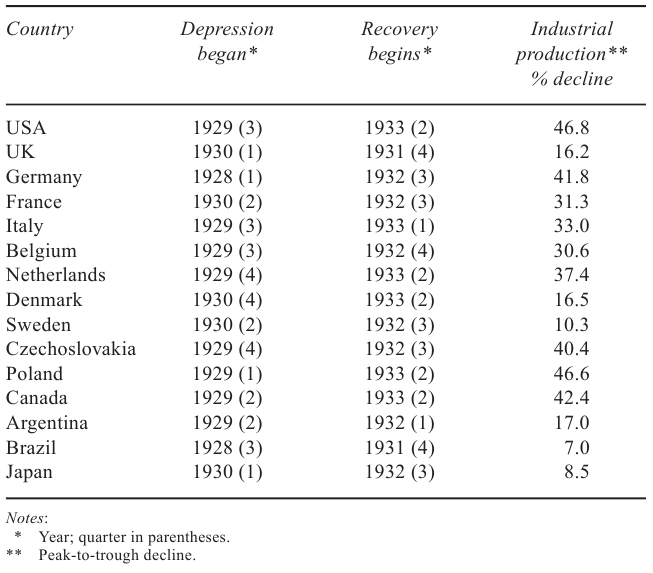
\includegraphics[width=0.55\textwidth]{./figures/aula4_fig0}
        \caption{Grande Depressão. Fonte: Romer (2004).}
        \label{aula4_fig0}
    \end{figure}
\end{frame}

\begin{frame}{A Grande Depressão da década de 1930}
    \begin{itemize}
        \item Grande Depressão: catástrofe econômica mais significativa a afetar economias capitalistas no século XX
        \bigskip
        \item A significância política e econômica deste acontecimento é refletida na agenda de pesquisa contínua e crescente deste evento histórico traumático
        \bigskip
        \item Extensão e magnitude da depressão pode ser vista nos dados da Tabela anterior
    \end{itemize}
\end{frame}

\begin{frame}
    {A Grande Depressão da década de 1930}
    \begin{itemize}
        \item Como explicar a queda acentuada no nível de atividade econômica agregado?\bigskip
        \item Pré-1930: visão dominante era de tradição clássica\bigskip
        \item \hlight{Teorema da mão invisível:} comportamento maximizador de utilidade e lucros de agentes econômicos racionais operando sob condições de mercados competitivos irá, via mecanismo da `mão invisível', traduzir as atividades de milhões de indivíduos em um ótimo social\bigskip
        \item Viés para \emph{laissez-faire} e visão clássica traduzida na Lei de Say (negando a possibilidade de super(sub)produção generalizada)\bigskip        
    \end{itemize}
\end{frame}

\begin{frame}{A Grande Depressão da década de 1930}
    \begin{itemize}
        \item Principal diagnóstico à época era de inspiração austríaca
        \bigskip
        \item A crise sinalizava uma situação de sobre-investimento e má alocação de recursos, um estado que requeria, para sua solução, um processo de `liquidação': deflação de salários reais por um lado, e sanções às firmas que engajaram em decisões erradas de investimento
        \bigskip
        \item O moto, portanto, era de flexibilização
        \bigskip
        \item Quanto mais flexíveis fossem preços e salários, mais rápido esse processo de liquidação terminaria e as condições de prosperidade seriam restauradas
        \bigskip
        \item No entanto, à medida que a depressão seguiu seu curso sem que a deflação de salários tivesse o efeito esperado, os economistas começaram a questionar as virtudes do \emph{laissez-faire} e a imaginar se os governos deveriam engajar de maneira mais ativa na estabilização da economia
    \end{itemize}
\end{frame}

\begin{frame}{A Grande Depressão da década de 1930}    
    \begin{figure}
        \centering
        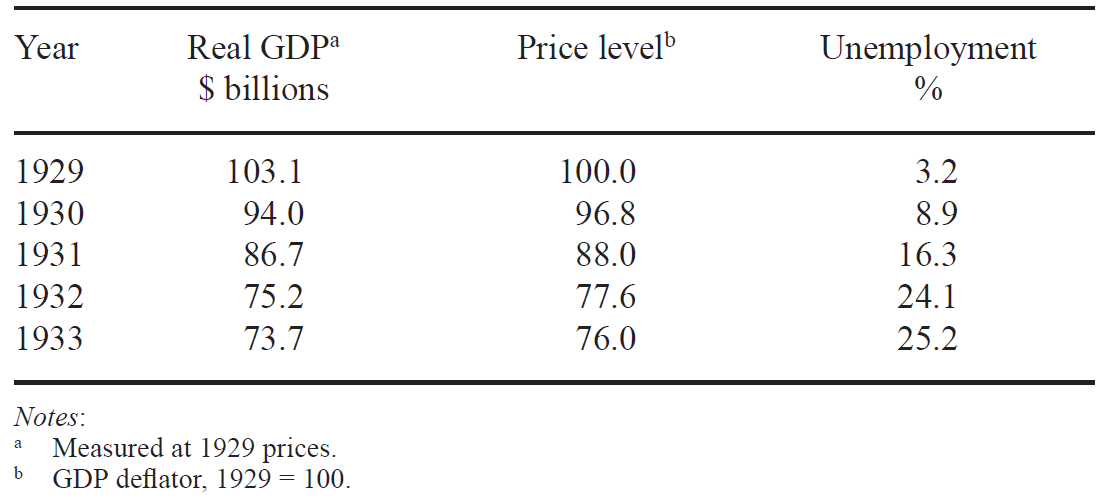
\includegraphics[width=0.9\textwidth]{./figures/aula4_fig1}
        \caption{PIB, preços e desemprego: EUA (1929-1933). Fonte: Snowdon e Vane (2005).}
        \label{fig1}
    \end{figure}
\end{frame}

\begin{frame}{A Grande Depressão da década de 1930}
    \begin{itemize}        
        \item Economistas, de maneira geral, concluíram que as prováveis causas da Grande Depressão envolvem a interação de vários fatores que levaram a uma drástica redução na demanda agregada\bigskip
        \item A Figura anterior apresenta fortes evidências que suportam a hipótese de um forte choque adverso de demanda agregada
        \bigskip
        \item Há um forte movimento procíclico do nível de preços, isto é, o nível de preços está decrescendo à medida que o PIB contrai
        \bigskip
        \item Note, ainda, o aumento considerável na taxa de desemprego
    \end{itemize}
\end{frame}

\begin{frame}{A Grande Depressão da década de 1930}
    \begin{itemize}
        \item Os dados consolidados por Bernanke e Carey (1996) mostram, ainda, que na grande maioria dos países houve um movimento contracíclico do salário real
        \bigskip
        \item Este padrão emergiria em resposta a um choque de demanda agregada naqueles países em que a deflação de preços viesse a exceder a deflação de salários
        \bigskip
        \item Portanto, Bernanke e Carey concluem que a evidência de ``uma curva de oferta agregada não-vertical na era da Depressão é forte'' (Bernanke e Carey, 1996)
    \end{itemize}
\end{frame}

\begin{frame}{A Grande Depressão da década de 1930}
    \begin{figure}
        \centering
        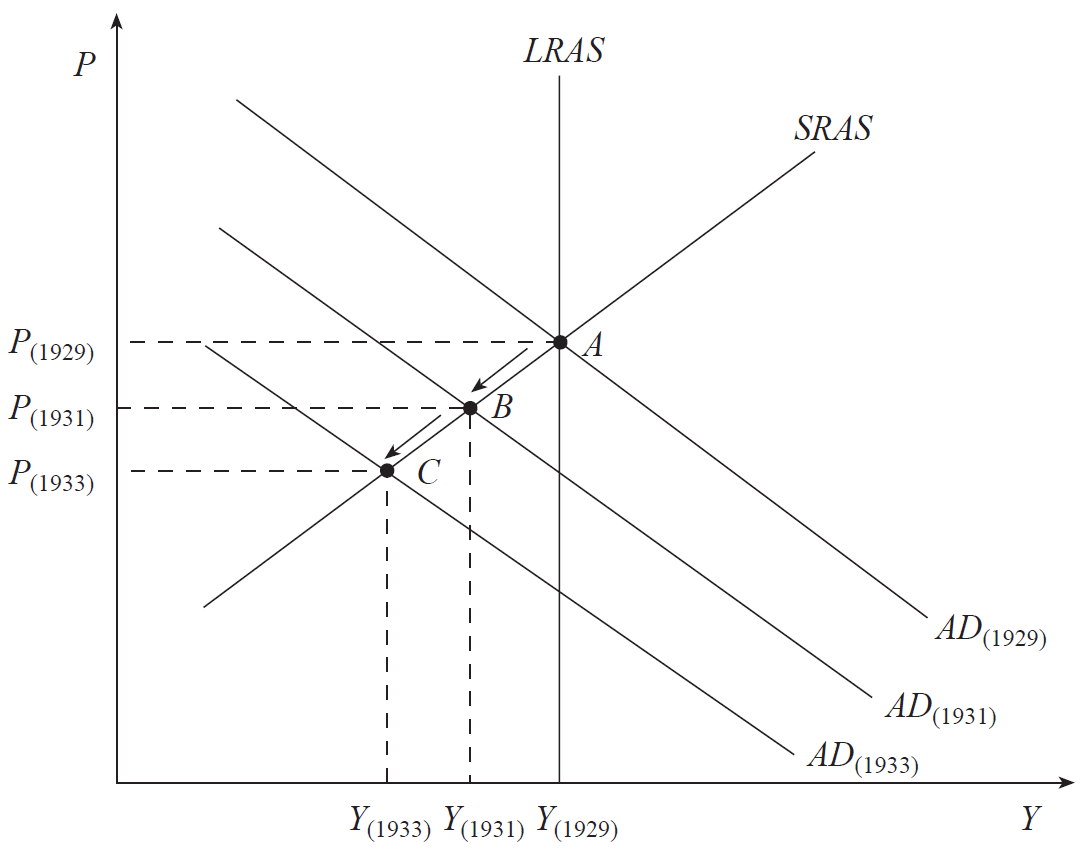
\includegraphics[width=0.55\textwidth]{./figures/aula4_fig2}
        \caption{Deficiência de demanda agregada - EUA (1929-33). Fonte: Snowdon e Vane (2005).}
        \label{fig2}
    \end{figure}
\end{frame}

\begin{frame}{A Grande Depressão da década de 1930}
    \begin{itemize}
        \item A Figura anterior ilustra essa situação para a economia dos EUA no período 1929-1933 usando o diagrama OA-DA
        \bigskip
        \item A queda significativa de demanda agregada é evidenciada pelo deslocamento da curva de Demanda Agregada para a esquerda durante este período
        \bigskip
        \item Note que uma combinação de queda do nível de preços e PIB não pode emergir de um choque adverso de oferta agregada - isso reduziria o PIB e aumentaria o nível de preços
    \end{itemize}
\end{frame}

\section{Programa de pesquisa}
\subsection{Motivação}
\begin{frame}{Motivação}
    \begin{itemize}
        \item O objetivo de Keynes com a publicação da Teoria Geral era identificar as causas do desemprego em massa que afetou todas as economias desenvolvidas nos anos da Grande Depressão
        \bigskip
        \item A década de 1930 foi, também, um período no qual a Rússia apresentava fortes resultados econômicos, o que poderia ter um efeito de possíveis vitórias eleitorais de partidos de vertentes comunistas (ou sua tomada de poder por vias menos ortodoxas)
        \bigskip
        \item Em resumo, a sobrevivência do sistema capitalista estava em cheque, tanto econômico quanto politicamente, e Keynes tinha ciência da necessidade de mudanças consideráveis em seu funcionamento: ``\emph{para salvar a civilização ocidental da enorme maré de barbárie que o colapso econômico estava trazendo}'' (Skidelsky, 1992)
    \end{itemize}
\end{frame}

\begin{frame}{Motivação}
    \NB{Os regimes autorit\'{a}rios contempor\^{a}neos parecem resolver o problema do desemprego \`{a} custa da efici\^{e}ncia e da liberdade. \'{E} certo que o mundo n\~{a}o tolerar\'{a} por muito mais tempo o desemprego que, \`{a} parte curtos intervalos de excita\c{c}\~{a}o; \'{e} uma consequ\^{e}ncia – e na minha opini\~{a}o uma consequ\^{e}ncia inevit\'{a}vel – do capitalismo individualista do nosso tempo. Mas pode ser poss\'{i}vel curar o mal por meio de uma an\'{a}lise correta do problema, preservando ao mesmo tempo a efici\^{e}ncia e a liberdade
    
    \begin{flushright}
        (Keynes, 1936).
        \end{flushright}}
\end{frame}

\begin{frame}{Motivação}
    \begin{itemize}
        \item Havia, portanto, um descolamento entre as implicações de política econômica derivadas da teoria estabelecida à época e a intuição dos formuladores de política de que um outro caminho deveria ser seguido
        \bigskip
        \item O projeto de Keynes com a Teoria Geral era, portanto, remover essa contradição ao fornecer um argumento teórico que desse fundamentos à intuição destes formuladores
    \end{itemize}
\end{frame}

\begin{frame}{Motivação}
    \begin{itemize}
        \item O aspecto mais revolucionário da obra de Keynes, que pode ser detectado nos seus escritos de meados de 1920 em diante, era sua mensagem clara e inequívoca com relação ao nível geral de emprego e produto de que não havia uma ``mão-invisível'' canalizando os interesses próprios dos agentes para algum nível ótimo social
        \bigskip
        \item Apesar de esta visão emergir repetidamente em suas críticas às políticas adotadas no UK ao longo da década de 20, muitas das suas recomendações de política econômica não continham uma estrutura teórica pela qual podiam ser logicamente derivadas
        \bigskip
        \item E.g.: em 1929, Keynes argumentava em favor de programas governamentais de estímulos de demanda financiados via déficit público em suporte ao programa liberal de recuperação de Lloyd George. Mas o fez sem uma teoria de demanda efetiva e mecanismos de multiplicadores que são fundamentais para seu argumento.
    \end{itemize}
\end{frame}

\subsection{O programa de pesquisa de Keynes}
\begin{frame}{O programa de pesquisa de Keynes}
    \begin{itemize}
        \item Nos próximos slides apresentaremos um sumário do programa de pesquisa de Keynes contido na Teoria Geral.
    \end{itemize}
\end{frame}

\begin{frame}{O programa de pesquisa de Keynes}
        \begin{enumerate}
            \item O objetivo de Keynes era demonstrar a possibilidade de existência teórica de \textcolor{blue}{desemprego involuntário}\bigskip
            \begin{itemize}
                \item Fenômeno cuja existência no mundo real é convincente, especialmente na Grande Depressão, para o qual a teoria econômica não admitia a existência\medskip
                \item Divisão do desemprego em duas categorias: fricional (normal) e involuntário (anormal)\medskip
                \item O desemprego involuntário, para Keynes, viola o segundo postulado clássico: igualdade entre utilidade marginal do consumo e desutilidade marginal do trabalho\medskip
                \item Na terminologia moderna, tomando a derivação padrão da curva de oferta de trabalho, o critério para existência de desemprego involuntário é que no período de fechamento de transações, alguns agentes se encontram excluídos da participação no mercado de trabalho dado o fato de que o salário de mercado é mais alto que seu salário de reserva
            \end{itemize}            
        \end{enumerate}
\end{frame}

\begin{frame}{O programa de pesquisa de Keynes}
  \begin{itemize}
      \item Isso significa que os agentes desempregados, ao contrário dos empregados, não conseguem realizar seus planos ótimos - estado de `desequilíbrio individual'\bigskip
      \item Esse resultado implica que os agentes são heterogêneos: trabalhadores desempregados derivam uma utilidade imediata inferior às dos agentes empregados\bigskip
      \item Essa é uma situação de um mercado de trabalho que apresenta um excesso de oferta de trabalho ou, em outras palavras, um racionamento de trabalho
  \end{itemize}
\end{frame}

\begin{frame}{O programa de pesquisa de Keynes}
  \begin{enumerate}    
  \item[2.] A teoria vigente da época argumentava que o desemprego era causado por rigidez de salários. Keynes desejava descartar essa visão. Ou seja, ele desejava exonerar a rigidez de salários da responsabilidade da existência de desemprego involuntário\bigskip
  
  \item[3.] O interesse de Keynes no desemprego involuntário decorria de sua conjectura de que este fenômeno expressa alguma falha nas economias capitalistas, um problema sistêmico que afeta o funcionamento de economias decentralizadas. Mais especificamente, ele desejava relacionar o desemprego involuntário com uma deficiência de demanda agregada com relação ao produto agregado o que estava, por sua vez, associado com algum vazamento do setor produtivo em direção ao setor financeiro. A implicação disso é que a interpretação otimista de economias de mercado dos economistas desde Adam Smith deve ser atenuada.
  \end{enumerate}
\end{frame}

\begin{frame}{O programa de pesquisa de Keynes}
    \begin{enumerate}    
        \item[4.] No prefácio da edição francesa de 1939, Keynes escreveu: ``Dei à minha teoria o nome de teoria \emph{geral}. Com isso quero dizer que estou preocupado principalmente com o comportamento do sistema econômico como um todo''\bigskip
        \begin{itemize}
            \item Em outras palavras, o desemprego involuntário deve ser considerado em termos de equilíbrio geral: mas sua origem deve ser identificada em outras partes da economia que não o mercado de trabalho:\medskip
            \NB{\emph{Eu sustento que o sal\'{a}rio real [...] n\~{a}o \'{e} determinado primordialmente pelos ``ajustes salariais'' [...] mas pelas outras for\c{c}as do sistema, algumas das quais (especialmente a rela\c{c}\~{a}o entre a curva da efici\^{e}ncia marginal do capital e a taxa de juros) o professor Pigou n\~{a}o incluiu.} (Keynes, 1936 - Ap\^{e}ndice Cap. 19).}\medskip
            \item No entanto, a decisão de Keynes de adotar uma perspectiva de interdependência não deve ser interpretada como uma adesão à abordagem de equilíbrio geral de Walras\medskip
            \item Para ele, o caminho a ser tomado era generalizar a análise de Marshall
        \end{itemize}        
    \end{enumerate}
\end{frame}

\begin{frame}{O programa de pesquisa de Keynes}
    \begin{enumerate}        
        \item[5.] Ao invés de adotar a linha de argumento de competição imperfeita que ganhava popularidade em Cambridge, Keynes desejava usar o arcabouço teórico de competição perfeita - talvez porque ele associasse competição imperfeita com conluio, sindicatos, etc., enquanto ele queria trazer algo mais profundo para a análise\bigskip
        \item[6.] A solução para o desemprego involuntário proposta por Keynes foi uma ativação de demanda induzida pelo estado, combinada com uma política de juros baixos e algumas doses de redistribuição de renda. Para Keynes, essas medidas não estão relacionadas com a introdução de algum tipo de socialismo mas, sim, para preservar o capitalismo democrático. Portanto, sua teoria pode ser caracterizada como \textcolor{blue}{conservadorismo moderado}
    \end{enumerate}
\end{frame}

\begin{frame}{O programa de pesquisa de Keynes}
    \begin{enumerate}        
        \item[7.] Após algumas ponderações, Keynes decidiu desenvolver sua linha de argumentação dentro dos cânones da teoria existente, i.e., a teoria Marshalliana. Ou seja, ele desejava defender suas alegações alterando minimamente a teoria bem estabelecida à época
    \end{enumerate}
\end{frame}

\section{Principais proposições}
\begin{frame}{Teoria Geral: principais proposições}
    \begin{itemize}
        \item O principal objetivo da Teoria Geral do Emprego, do Juro e da Moeda é ``\textcolor{blue}{descobrir o que, em um dado sistema econômico, determina em um momento preciso a renda nacional e  (o que vem a ser quase a mesma coisa) o volume de emprego que lhe corresponde}'' (Keynes, 1936)
        \bigskip
        \item Já que no arcabouço teórico desenvolvido por Keynes, ``a renda nacional depende do volume do emprego''
        \bigskip
        \item Outro objetivo de Keynes era demonstrar que o equilíbrio macroeconômico é consistente com a existência de \textcolor{blue}{desemprego involuntário}
    \end{itemize}
\end{frame}

\begin{frame}{Teoria Geral: principais proposições}
    \begin{itemize}
        \item A novidade teórica e proposição central da obra é o \textcolor{blue}{princípio da demanda efetiva}, combinado com o papel equilibrador de variações na quantidade (renda nacional) ao invés de preços
        \bigskip
        \item A ênfase dada ao ajuste via quantidade ao invés de preços está em nítido contraste com o modelo clássico que estudamos anteriormente
        \bigskip
        \item Além disso, contrasta também com o pensamento de Keynes anterior à publicação da Teoria Geral, contido na obra \emph{Treatise on Money} (Tratado sobre a moeda), de 1930
        \bigskip
        \item Neste trabalho, diferenças entre decisões de poupança e de investimento levam a oscilações no nível de preços
    \end{itemize}
\end{frame}

\begin{frame}{Teoria Geral: principais proposições}
    \begin{itemize}
        \item O princípio da demanda efetiva afirma que em uma economia fechada com capacidade ociosa, o nível de produto (e, portanto, de emprego) é determinado pelos gastos agregados planejados
        \bigskip
        \item Estes gastos agregados planejados são compostos por dois componentes: gastos de consumo por parte das famílias ($C$) e gastos de investimento pelas firmas ($I$)
        \bigskip
        \item Na Teoria Geral não há uma análise explícita a respeito dos efeitos de variações nos gastos estimulados diretamente pelos gastos do governo ou indiretamente via mudanças na tributação
    \end{itemize}
\end{frame}

\begin{frame}{Teoria Geral: principais proposições}
    \begin{itemize}
        \item Portanto, na Teoria Geral, há apenas dois setores (famílias e firmas), e o gasto planejado é dado por:
        \begin{equation}
            E = C + I.
            \label{eq1}
        \end{equation}
        \bigskip
        \item No modelo clássico, como vimos nas aulas passadas, consumo, poupança e investimento são funções da taxa de juros
        \bigskip
        \item Já no modelo de Keynes, os gastos com consumo são endógenos e essencialmente passivos, dependendo do nível de renda ao invés da taxa de juros
        \bigskip
        \item A \textcolor{blue}{teoria do consumo} de Keynes, que veremos adiante, desenvolve esta relação entre consumo e renda
    \end{itemize}
\end{frame}

\begin{frame}{Teoria Geral: principais proposições}
    \begin{itemize}
        \item Os gastos com investimento dependem da rentabilidade esperada do investimento e da taxa de juros (que representa o custo dos fundos emprestáveis)
        \bigskip
        \item Keynes denomina os lucros esperados de \textcolor{blue}{eficiência marginal do capital}
        \bigskip
        \item Portanto, na teoria de Keynes, o nível de emprego torna-se dependente de um fator instável, o gasto com investimentos, que é suscetível a flutuações amplas e repentinas
    \end{itemize}
\end{frame}

\begin{frame}{Teoria Geral: principais proposições}
    \begin{itemize}
        \item A dependência do produto e do emprego com relação ao investimento não seria tão importante se os gastos com investimentos fossem estáveis
        \bigskip
        \item No entanto, as decisões de investimento são complicadas pois a aquisição de máquinas e equipamentos e/ou novas plantas de produção são tomadas em um período para produzir bens finais que serão vendidos em um futuro que é, inevitavelmente, incerto
        \bigskip
        \item Portanto, as \textcolor{blue}{expectativas} dos agentes acerca dos níveis futuros de demanda e custos são envolvidas nos cálculos em seus processos decisórios. O que possibilita que, na terminologia de Keynes, ``esperanças e medos'' influenciem as decisões tomadas
    \end{itemize}
\end{frame}

\begin{frame}{Teoria Geral: principais proposições}
    \begin{itemize}
        \item De fato, em um artigo escrito em resposta a alguns críticos que foi publicado um ano após a Teoria Geral, Keynes declarou que a mensagem central do livro era a ``incerteza radical que está envolvida nas decisões de investimento'' (Keynes, 1937 - The general theory of unemployment.)
        \bigskip
        \item \textcolor{blue}{Incerteza} só está presente em um capítulo da Teoria Geral, Capítulo 12, que lida com as expectativas de longo prazo
        \bigskip
        \item Neste capítulo, Keynes introduz a famosa expressão \textcolor{blue}{``animal spirits''} para se referir a um ``instinto espontâneo de agir, em vez de não fazer nada, e não o resultado de uma média ponderada de lucros quantitativos multiplicados pelas probabilidades quantitativas''
    \end{itemize}
\end{frame}

\begin{frame}{Teoria Geral: principais proposições}
    \begin{itemize}
        \item Portanto, dada a volatilidade das expectativas, frequentemente impulsionada por animal spirits, a rentabilidade esperada do capital também deve ser um fator altamente instável
        \bigskip
        \item Como as decisões de investimento podem ser influenciadas por ondas de otimismo ou pessimismo irracionais (desvinculadas dos fundamentos econômicos), causando flutuações amplas no estado de confiança dos negócios, isso levou Keynes a questionar a eficácia dos ajustes nas taxas de juros como forma de influenciar o volume de investimentos
    \end{itemize}
\end{frame}

\begin{frame}{Teoria Geral: principais proposições}
    \begin{itemize}
        \item \textcolor{blue}{As expectativas acerca da rentabilidade futura do investimento são muito mais importantes que a taxa de juros em relacionar o futuro com o presente}, isso porque:\bigskip
    \end{itemize}
    \NB{dada a psicologia das massas (do p\'{u}blico), o n\'{i}vel de produto e emprego como um todo depende do n\'{i}vel de investimento, e s\~{a}o estes fatores que determinam a taxa de investimento os menos confi\'{a}veis, dado que s\~{a}o eles que s\~{a}o influenciados pelas nossas vis\~{o}es do futuro acerca do qual sabemos t\~{a}o pouco.
        \medskip
        \begin{flushright}
        (Keynes, 1936).
        \end{flushright}}
\end{frame}

\begin{frame}{Teoria Geral: principais proposições}
    \begin{itemize}
        \item A `extrema precariedade' do conhecimento que uma firma possui a respeito do retorno esperado de uma decisão de investimento está no centro da explicação de Keynes sobre os ciclos de negócios
        \bigskip
        \item Em sua análise de instabilidade, `flutuações violentas' na eficiência marginal do capital formam os choques que deslocam a \textcolor{blue}{demanda agregada real}
        \bigskip
        \item Ou seja, a principal fonte de flutuações econômicas vem do lado real da economia (como descrito pela curva IS)
    \end{itemize}
\end{frame}

\begin{frame}{Teoria Geral: principais proposições}
    \begin{itemize}
        \item Capítulo 12, no qual é discutido o papel das expectativas de longo prazo, é ``estranho'' ao restante do livro
        \bigskip
        \item No restante da obra, Keynes separa o funcionamento de curto e longo-prazo de uma economia, focando na questão mais tratável, isto é, a determinação de curto prazo do nível de emprego
        \bigskip
        \item E o faz baseando sua análise na hipótese de informação perfeita - no espectro oposto da ideia de animal spirits
    \end{itemize}
\end{frame}

\begin{frame}{Teoria Geral: principais proposições}
    \begin{itemize}
        \item Para sua análise da \textcolor{blue}{função consumo}, Keynes desenvolveu o conceito de propensão marginal a consumir, que tem um papel fundamental na determinação da magnitude do multiplicador
        \bigskip
        \item Por causa da presença de um processo multiplicador, qualquer distúrbio nos gastos com investimentos terá um impacto amplificado sobre o produto agregado
        \bigskip
        \item Seja $c$ a propensão marginal a consumir das famílias ($c \equiv dC/dY$) e $a$ o nível de consumo autônomo, a equação comportamental para o consumo é dada por:
        \begin{equation}
            C = a + cY.
            \label{eq2}
        \end{equation}
    \end{itemize}
\end{frame}

\begin{frame}{Teoria Geral: principais proposições}
    \begin{itemize}
        \item A condição de equilíbrio é, portanto:
        \begin{equation}
            Y = \underbrace{a + cY}_{\text{Consumo}} + \overbrace{I}^{\text{Investimento}}.
            \label{eq3}
        \end{equation}
        \bigskip
        \item A equação em forma reduzida será dada, então, por:
        \begin{equation}
            Y = \frac{1}{1 - c}(a + I) = \kappa (a + I),
            \label{eq4}
        \end{equation}
        onde $\kappa \equiv 1/(1 - c)$ representa o multiplicador Keynesiano
    \end{itemize}
\end{frame}

\begin{frame}{Teoria Geral: principais proposições}
    \begin{itemize}
        \item Segue, portanto, que para uma dada variação nos gastos com investimentos, \emph{ceteris paribus}, teremos:
        \begin{equation}
            dY = \kappa dI.
            \label{eq5}
        \end{equation}
        \bigskip
        \item Ou seja, a renda agregada (produto agregado) varia por um múltiplo da mudança nos gastos com investimento
        \bigskip
        \item Keynes define o multiplicador do investimento, $\kappa$, como a taxa de variação na renda em resposta a variações no gasto autônomo que este gera: ``\emph{quando há um aumento no investimento agregado, a renda aumentará em uma magnitude igual a $\kappa$ vezes o aumento no investimento}'' (Keynes, 1936)
    \end{itemize}
\end{frame}

\begin{frame}{Teoria Geral: principais proposições}
    \begin{itemize}
        \item \emph{Ceteris paribus}, o multiplicador será maior quanto menor for a propensão marginal a poupar
        \bigskip
        \item O efeito multiplicador mostra que para um deslocamento no componente autônomo da demanda ($dI$), a renda inicialmente aumentará em uma magnitude equivalente
        \bigskip
        \item Este aumento na renda, por sua vez, aumenta o consumo agregado em $cdI$
        \bigskip
        \item Este aumento no consumo leva a um aumento de igual magnitude na renda que, na segunda iteração, leva a um novo aumento nos gastos de $c(cdI)$, o que leva a um novo aumento nos gastos e na renda
        \bigskip
        \item Portanto, temos uma série geométrica infinita tal que o efeito total de uma variação autônoma da demanda sobre o produto é dado por:
        \begin{equation}
            dY = dI + cdI + c^2dI + c^3 dI + \dots = \frac{1}{1 - c} dI.
            \label{eq6}
        \end{equation}
    \end{itemize}
\end{frame}

\begin{frame}{Teoria Geral: principais proposições}
    \begin{itemize}
        \item Ao longo da análise anterior, assumimos uma economia com capacidade ociosa, onde as firmas são capazes de responder à demanda extra produzindo mais produtos
        \bigskip
        \item Dado que um nível de produção maior requer mais insumo trabalho, o multiplicador do produto implica a existência de um multiplicador do emprego (Kahn, 1931)
        \bigskip
        \item Portanto, um aumento no gasto autônomo leva a um aumento no produto e emprego agregados
    \end{itemize}
\end{frame}

\begin{frame}{Teoria Geral: principais proposições}
    \begin{itemize}
        \item Se considerarmos uma economia iniciando em uma posição abaixo do nível de pleno emprego, suponha que ocorra um aumento na quantidade de investimento autônomo nesta economia
        \bigskip
        \item O aumento nos gastos com investimento resultará em um aumento do emprego nas firmas produtoras de bens de capital
        \bigskip
        \item Estes novos trabalhadores empregados nas indústrias de bens de capital irão gastar parte de sua renda em bens de consumo e poupar o restante
        \bigskip
        \item O aumento da demanda por bens de consumo, por sua vez, leva a um aumento do emprego nas indústrias de bens de consumo e resultará em novas rodadas de dispêndio
        \bigskip
        \item Consequentemente, um aumento inicial no investimento autônomo produz um aumento mais que proporcional na renda agregada
        \bigskip
        \item O mesmo processo multiplicador se aplica seguindo uma variação não apenas no gasto com investimentos mas, também, no componente autônomo do consumo das famílias
    \end{itemize}
\end{frame}

\begin{frame}{Teoria Geral: principais proposições}
    \begin{itemize}
        \item Em termos do modelo da cruz Keynesiana proposto por Paul Samuelson, um multiplicador maior será representado por uma agenda de gastos agregados mais inclinada, e vice-versa.
    \end{itemize}
    \begin{figure}
        \centering
        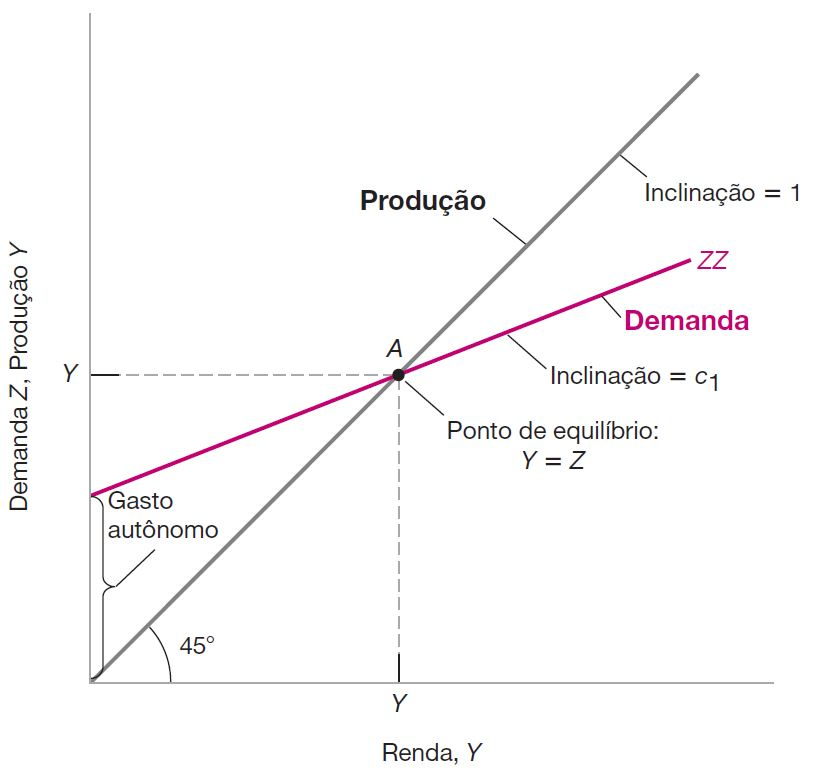
\includegraphics[width=0.4\textwidth]{./figures/aula4_fig3}
        \caption{Diagrama da cruz Keynesiana. Fonte: Blanchard (2017).}        
    \end{figure}
\end{frame}

\begin{frame}{Teoria Geral: principais proposições}
    \begin{itemize}
        \item Já no modelo Keynesiano IS-LM, o multiplicador afeta a inclinação da curva IS. A curva IS será menos inclinada quanto maior for o multiplicador, e vice-versa.
    \end{itemize}
    \begin{figure}
        \centering
        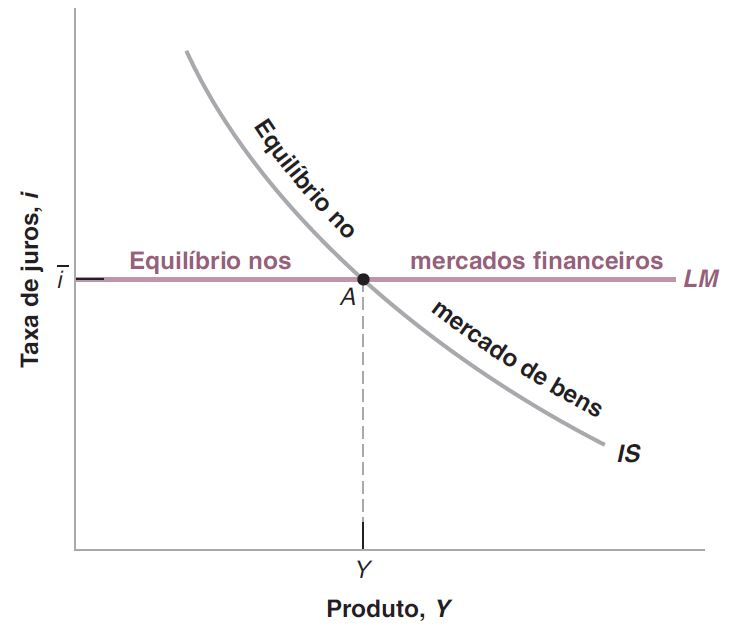
\includegraphics[width=0.4\textwidth]{./figures/aula4_fig4}
        \caption{Diagrama IS-LM. Fonte: Blanchard (2017).}        
    \end{figure}
\end{frame}

\begin{frame}{Teoria Geral: principais proposições}
    \begin{itemize}
        \item Keynes tinha ciência dos vários fatores que poderiam limitar a magnitude do efeito multiplicador dos seus programas de gastos públicos propostos
        \bigskip
        \item Incluindo o efeito de ``um aumento da taxa de juros'' a não ser que ``a autoridade monetária tome medidas contrárias'', criando um efeito deslocamento (\emph{crowding-out}) do investimento em outras direções
        \bigskip
        \item O potencial para um efeito adverso sobre o nível de ``confiança'' dos agentes econômicos
        \bigskip
        \item E o ``vazamento'' (\emph{leakage}) dos gastos tanto em direção a impostos quanto para importações em uma economia aberta
        \bigskip
        \item Já para o caso de uma economia operando em pleno emprego, Keynes reconhece que qualquer aumento no investimento irá ``criar uma tendência nos preços monetários de crescer de forma ilimitada, independente da propensão marginal a consumir'' (Keynes, 1936)
    \end{itemize}
\end{frame}

\begin{frame}{Teoria Geral: principais proposições}
    \begin{itemize}
        \item A determinação da taxa de juros na teoria de Keynes também marca um claro rompimento com o modelo clássico
        \bigskip
        \item Keynes rejeitava a ideia de que a taxa de juros fosse determinada pelas forças reais de produtividade marginal do capital e parcimônia
        \bigskip
        \item Na Teoria Geral, a taxa de juros é um fenômeno puramente monetário determinada pela \textcolor{blue}{preferência pela liquidez} (demanda por moeda) do público de forma conjunta com a oferta de moeda determinada pelas autoridades monetárias
        \bigskip
        \item Além do motivo transação para reter moeda, Keynes adicionou os motivos precaução e especulação, sendo que este último é sensível a variações na taxa de juros
    \end{itemize}
\end{frame}

\begin{frame}{Teoria Geral: principais proposições}
    \begin{itemize}
        \item Keynes rejeitou a ideia clássica de que os juros representam uma recompensa para os agentes em postergar o consumo presente
        \bigskip
        \item Para ele, a taxa de juros é uma recompensa por se desfazer de um ativo líquido ou não acumular por um período especificado
        \bigskip
        \item Em um mundo caracterizado pela incerteza, sempre haverá um motivo especulação para reter moeda em comparação com outros ativos financeiros (como títulos)
        \bigskip
        \item E na visão de Keynes, a preferência pela liquidez sempre terá uma influência maior sobre a taxa de juros do que as decisões de poupança
        \bigskip
        \item Se a preferência pela liquidez por parte dos agentes pode variar, isso compromete o postulado clássico relacionado à estabilidade de função de demanda por moeda
        \bigskip
        \item Isso, por sua vez, implica que a velocidade de circulação da moeda provavelmente varia
    \end{itemize}
\end{frame}

\begin{frame}{Teoria Geral: principais proposições}
    \begin{figure}
        \centering
        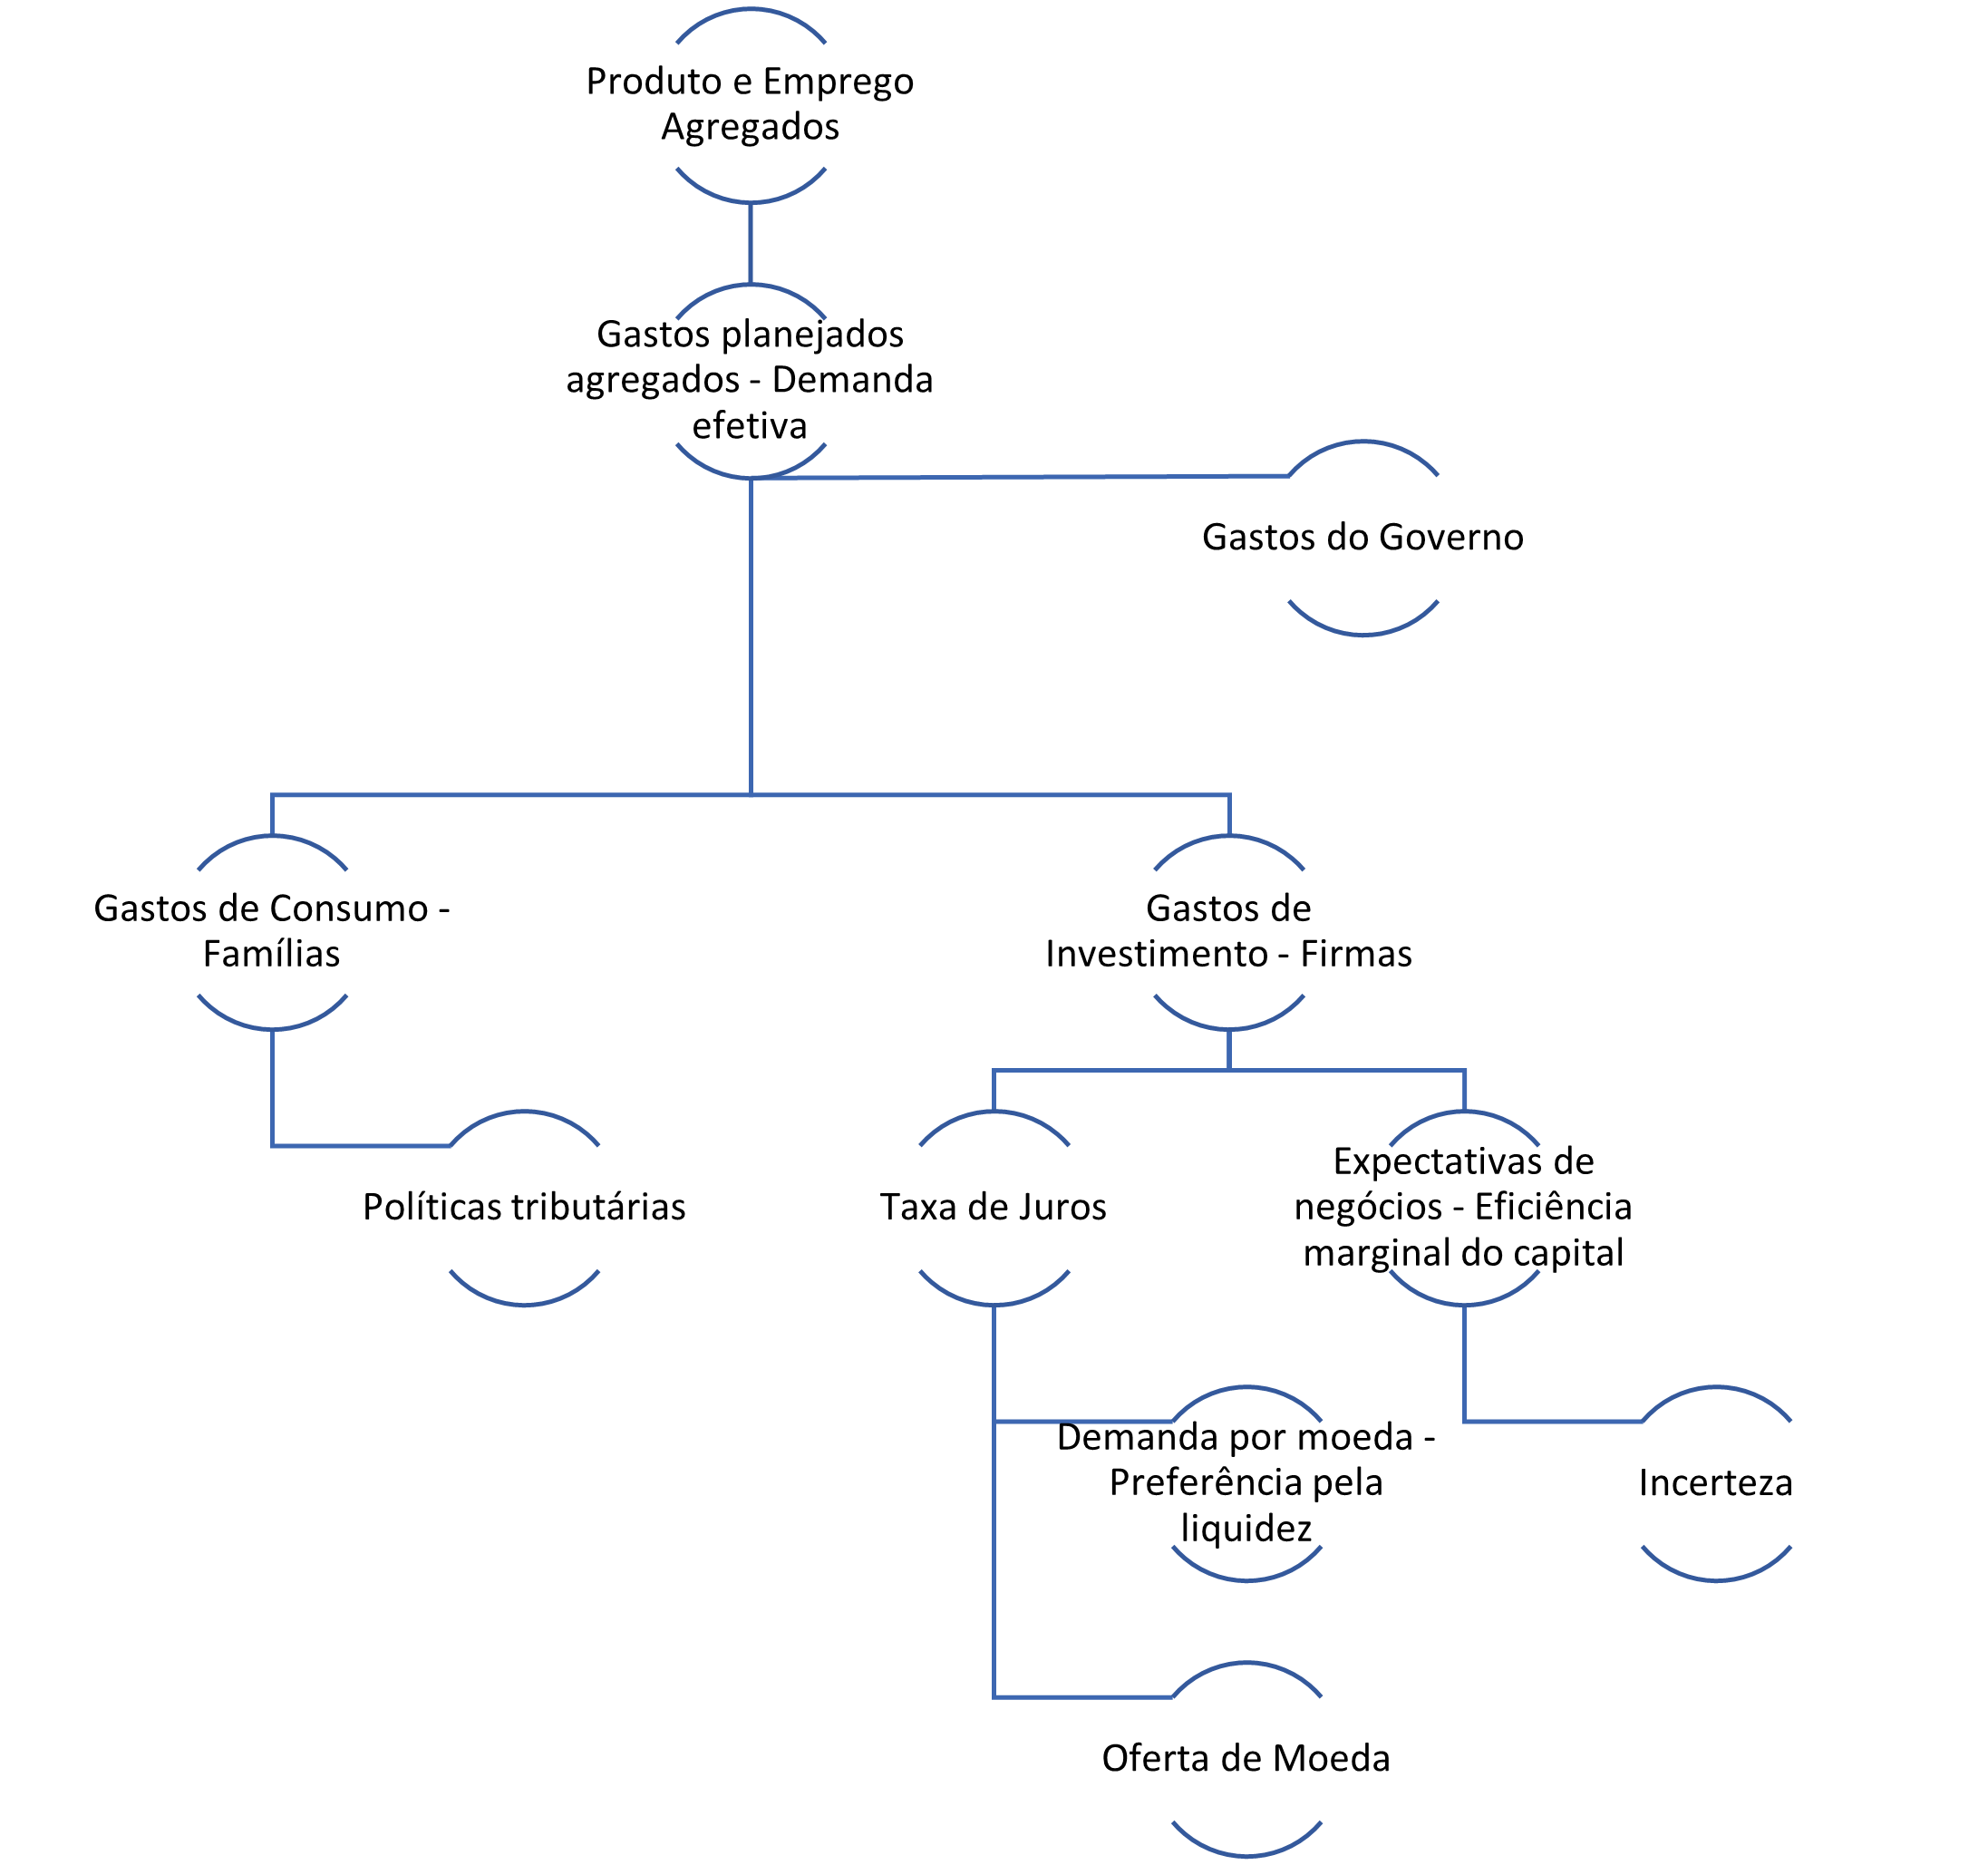
\includegraphics[width=0.5\textwidth]{./figures/aula4_fig5}
        \caption{Determinação do produto e emprego. Fonte: Snowdon e Vane (2005).}        
    \end{figure}
\end{frame}

\begin{frame}{Teoria Geral: principais proposições}
    \begin{itemize}
        \item A estrutura básica da teoria da demanda efetiva de Keynes é representada na figura anterior
        \bigskip
        \item Podemos ver que a dependência do produto e emprego agregados do fator dispêndio agregado ($C + I$) cria um potencial de instabilidade no modelo, dado que os gastos com investimentos são tipicamente instáveis devido à influência das expectativas de negócios relacionadas a um futuro incerto
        \bigskip
        \item Um futuro incerto também cria um desejo por liquidez, de forma que variações na demanda por moeda, assim como mudanças na oferta monetária, podem influenciar o produto e o emprego
        \bigskip
        \item Portanto, \textcolor{blue}{no modelo de Keynes, a proposição clássica de neutralidade da moeda é rejeitada}
    \end{itemize}
\end{frame}

\begin{frame}{Teoria Geral: principais proposições}
    \begin{itemize}
        \item Para Keynes, um aumento na oferta de moeda, ao reduzir a taxa de juros, pode estimular os gastos agregados via um aumento no nível de investimentos e o efeito multiplicador subsequente
        \bigskip
        \item Essa relação pode ser representada da seguinte forma:
        \begin{equation}
            +\Delta M \rightarrow -\Delta r \rightarrow +\Delta I \rightarrow +\Delta Y, +\Delta L.
            \label{eq7}
        \end{equation}
    \end{itemize}
\end{frame}

\begin{frame}{Teoria Geral: principais proposições}
    \begin{itemize}
        \item A esta altura deve estar claro porque o livro de Keynes é entitulado \emph{Teoria Geral do Emprego, do Juro e da Moeda}
        \bigskip
        \item Para Keynes, era geral porque o equilíbrio de pleno emprego clássico é um caso especial de sua análise
        \bigskip
        \item E as ``características desse caso especial não são as da sociedade econômica em que realmente vivemos'' (Keynes, 1936)
        \bigskip
        \item No entanto, Keynes reconhecia que a potência da política monetária pode ser limitada, particularmente em um período de profunda recessão econômica: ``se nos vemos tentados a considerar a moeda como a bebida que estimula a atividade do sistema, não nos esqueçamos que podem surgir muitos percalços entre a taça e os lábios'' (Keynes, 1936)
    \end{itemize}
\end{frame}

\begin{frame}{Teoria Geral: principais proposições}
    \begin{itemize}
        \item Portanto, nos casos em que a política monetária é fraca ou ineficaz, os gastos agregados podem ser estimulados diretamente via gastos públicos ou indiretamente via mudanças na tributação que estimulem o consumo das famílias ao aumentar a renda disponível
        \bigskip
        \item Nas notas conclusivas da Teoria Geral, Keynes fornece alguns indícios de suas conclusões em termos de política econômica: ``O Estado deverá exercer uma influência orientadora sobre a propensão a consumir, em parte através de seu sistema de tributação, em parte por meio da fixação da taxa de juros e, em parte, talvez, recorrendo a outras medidas'' (Keynes, 1936)
    \end{itemize}
\end{frame}

\begin{frame}{Teoria Geral: principais proposições}
    \begin{itemize}
        \item Em nossos estudos sobre o modelo clássico, focamos em três aspectos daquela teoria:
        \bigskip
        \begin{enumerate}
            \item Teoria da determinação do emprego e produto agregados
            \medskip
            \item A Lei de Mercados de Say
            \medskip
            \item Teoria Quantitativa da Moeda
        \end{enumerate}
        \medskip
        \item Na próxima aula discutiremos, de maneira breve, como Keynes rejeita as idéias básicas relacionadas a cada um desses fundamentos da teoria clássica
    \end{itemize}
\end{frame}

\section{Paradoxo da poupança}
\begin{frame}{Paradoxo da poupança}
    \begin{itemize}
        \item Os aumentos nos níveis de poupança que seguiram a Crise Financeira Global de 2008-2009 e a pandemia recente reacenderam o interesse de economistas e formuladores de política econômica no paradoxo da poupança, formulado por Keynes na década de 1930
        \bigskip
        \item O \textcolor{blue}{paradoxo da poupança} afirma que um aumento na poupança não leva, naturalmente, a um aumento no nível de investimentos. O que pode levar ao que discutimos anteriormente, uma tendência crônica de que a propensão a poupar seja superior ao incentivo para investir
        \bigskip
        \item Pelo contrário, a \textcolor{blue}{poupança precaucionária} (\emph{precautionary savings}) - poupança adicional resultante de um futuro incerto - é prejudicial ao crescimento econômico dado que \emph{desloca} (\emph{crowds out}) o consumo e, portanto, diminui a demanda agregada
    \end{itemize}
\end{frame}

\begin{frame}{Paradoxo da poupança}
    \begin{itemize}
        \item A pandemia do COVID-19 causou um aumento sem precedentes nos níveis de poupança
        \bigskip
        \item Na UE, a taxa de poupança das famílias aumentou de 12,5\% para 17\%
        \bigskip
        \item Durante a CFG de 2008, o aumento foi de 12,5\% para 14\%
        \bigskip
        \item Mesmo que os motivos sejam diferentes agora, é óbvio que este aumento nos níveis de poupança não resulta em um aumento dos investimentos e do crescimento econômico
        \bigskip
        \item Dadas as expectativas pessimistas e incertezas nos mercados de trabalho e de créditos, é mais provável que essa poupança forçada acumulada durante as medidas de restrição será parcialmente transformada em poupança precaucionária
    \end{itemize}
\end{frame}

\begin{frame}{Paradoxo da poupança}
    \begin{itemize}
        \item Por estas razões, os formuladores de política econômica encoraja(ra)m fortemente o consumo assim que as condições sanitárias permitirem
        \bigskip
        \item Estas situações são similares àquelas enfrentadas por Keynes em 1931:
        \NB{There are today many well-wishers of their country who believe that the most useful thing which they and their neighbours can do to mend the situation is to save more than usual. […] It is utterly harmful and misguided – the very opposite of the truth.
        
        \begin{flushright}
            (Keynes, 1931 - Essays in Persuasion).
        \end{flushright}}
    \end{itemize}
\end{frame}

\begin{frame}{Paradoxo da poupança}
    \begin{itemize}
        \item Uma breve inspeção visual dos dados sugere que, de fato, a proporção dos depósitos de poupança com relação ao PIB aumentou mais naqueles países onde o PIB real apresentou um crescimento menor.
    \end{itemize}
    \begin{figure}
        \centering
        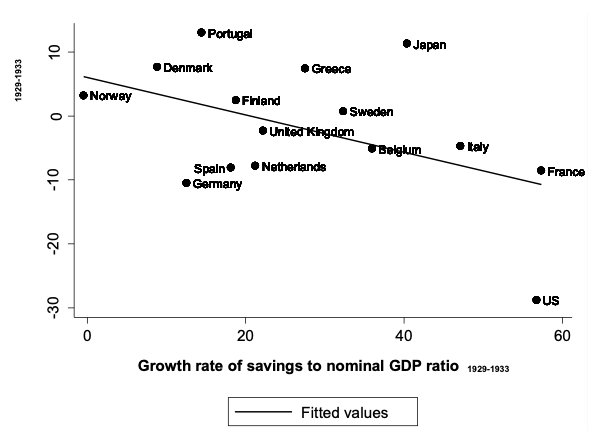
\includegraphics[width=0.5\textwidth]{./figures/aula4_fig6}
        \caption{Correlação entre o aumento na taxa de poupança e crescimento do PIB real durante a Grande Depressão, 1929-1933. Fonte: Degorce e Monnet (2020).}        
    \end{figure}
\end{frame}

\section{Bibliografia}
\begin{frame}{\emoji{books} Bibliografia}
    \begin{itemize}
        \item BERNANKE, B.S.; CAREY, K. Nominal wage stickiness and aggregate supply in the Great Depression, \emph{Quarterly Journal of Economics}, August/1996.\medskip
        \item DE VROEY, M. \emph{A History of Macroeconomics from Keynes to Lucas and Beyond}. Cambridge University Press, 2016.\medskip
        \item KEYNES, J.M. \emph{A teoria geral do emprego, do juro e da moeda}. São Paulo: Atlas, 1992. (Data do original em inglês: 1936).\medskip
        \item ROMER, C.D. The Great Depression, in \emph{Encyclopedia Britannica}, Upper Saddle River, NJ: Pearson Education, 2004.\medskip
        \item SKIDELSKY, R. \emph{John Maynard Keynes, Vol. 2: The Economist as Saviour 1920-1937}, London: Macmillan, 1992.\medskip
        \item SNOWDON, B.; VANE, H.R. \emph{Modern Macroeconomics: its Origins, Development and Current State}. Northampton, MA: Edward Elgar, 2005.
    \end{itemize}
\end{frame}
\end{document}